\chapter{Unité et diversité des langages}

\section{Des éléments communs}
Un langage de programmation sert à traduire des algorithmes pour les exécuter sur un ordinateur. Il est composé 
\begin{itemize}
    \item   d'un alphabet (ensemble de lettres et de symboles);
    \item   d'un vocabulaire (les \textit{mots-clés} du langage);
    \item   d'une grammaire (la \textit{syntaxe} du langage).
\end{itemize}

Les notions suivantes sont communes à l'immense majorité des langages :

\begin{itemize}
    \item   une \textit{instruction} est un ordre donné;
    \item   une \textit{variable} est un nom qui fait référence à une donnée manipulée par le programme et susceptible de changer au cours de celui-ci;
    \item   une \textit{constante} est un nom qui fait référence à une valeur immuable;
    \item   un \textit{type} qui sert à classifier une variable ou une constante et conditionne les opérations qu'il est possible d'effectuer;
    \item   la \textit{déclaration} consiste à renseigner le traducteur du programme sur la nature des données du programme (type, valeur).
    \item   les \textit{structures de contrôle} telles que le \textit{test} et les \textit{boucles}.
    \item   une \textit{fonction} (ou procédure, ou méthode) sert à isoler un fragment de programme pour pouvoir l'utiliser (éventuellement plusieurs fois) de manière paramétrée.
\end{itemize}

\section{Des différences}

\subsection{Différences formelles}

Tous les langages n'utilisent pas la même syntaxe. En examinant un même algorithme écrit dans plusieurs langages, on constate que 

\begin{itemize}
    \item   L'affectation peut être signifiée par \texttt{=} (comme en \textsc{Python}, \textsc{Basic}, \textsc{C}, \textsc{Fortran}...) ou par \texttt{:=} (\textsc{Ada}, \textsc{Algol}, \textsc{Go} pour partie...). On utilise aussi \texttt{<-} en \textsc{Caml}.
    \item   Les \textit{listes} (ou tableaux) sont très souvent indicées à partir de zéro... Mais pas toujours (\textsc{Fortran}, \textsc{Lua}).
    \item   Très souvent, les structures de contrôles sont délimitées par des accolades (\textsc{C}, \textsc{Java},  \textsc{Kotlin}...) ou par des \texttt{begin} et des \texttt{end} (\textsc{Ruby}, \textsc{Pascal}...). Parfois on utilise des variantes du \texttt{end} telles que \texttt{done}, \texttt{END-IF} ou \texttt{NEXT} pour signifier une fin de boucle « pour» .
\end{itemize}

Certains langages ont des syntaxes très similaires : le langage \textsc{C}, \textsc{Java} et \textsc{Javascript} par exemple (notamment le fait qu'un point-virgule termine une ligne).\\
D'autres ont une syntaxe et une mise en forme particulière, éloignée de tous les autres, comme le \textsc{Basic} ou le \textsc{Cobol}.

\subsection{Différences structurelles}

Certains langages obligent à déclarer le type des variables lors de leur création. C'est le cas de \textsc{C} ou \textsc{Java}. D'autres obligent même à renseigner les variables et leur type avant toute chose, comme \textsc{Ada}, \textsc{Algol}, \textsc{Cobol}. Ce n'est pas le cas en \textsc{Python} ou en \textsc{Ruby}.\\

Une autre différence majeure vient de la manière dont est traité le programme par le traducteur :

\begin{itemize}
    \item   En \textsc{C} ou en \textsc{C++}, le programme est transformé en \textit{langage-machine} par un \textit{compilateur}. L'intérêt est que l'on gagne en rapidité lors de l'exécution du programme.
    \item   En \textsc{Python} le programme est \textit{interprété}  lors de son exécution, ligne par ligne.
    \item   Beaucoup de langages utilisent un procédé hybride : le langage utilise une machine virtuelle, et les programmes sont compilés dans le langage de cette machine virtuelle, qui sera ensuite exécuté. La compilation peut être faite avant et le résultat stocké dans un fichier, ou bien être faite à la volée (\textit{Just In Time compilation}).
\end{itemize}



Chaque langage suit un ou plusieurs \textit{paradigmes} de programmation qui change radicalement la manière d'écrire les programmes.\\
Chaque langage suit un ou plusieurs \textit{paradigmes} de programmation qui change radicalement la manière d'écrire les programmes.\\
Nous avons vu la programmation \textit{impérative} (séquentielle, linéaire) où le programme effectue une liste d'instructions pas-à-pas. Il existe la programmation \textit{évènementielle} lors de laquelle on précise à \textsc{Processing} ce qu'il doit faire quand tel ou tel évènement se produit.\\
D'autres paradigmes de programmation telle la programmation \textit{orientée objet} ou la programmation \textit{fonctionnelle} sont très utilisés.

Enfin on distinguera des différences dans les contexte d'utilisation de chaque langages : il existe des langages généralistes, des langages qui sont censés être exécutés sur des « serveurs de pages web»  tels \textsc{PHP}, d'autres qui (à la base) ont été conçus pour être exécutés au sein même d'un navigateur (\textsc{Javascript}).

\begin{center}
    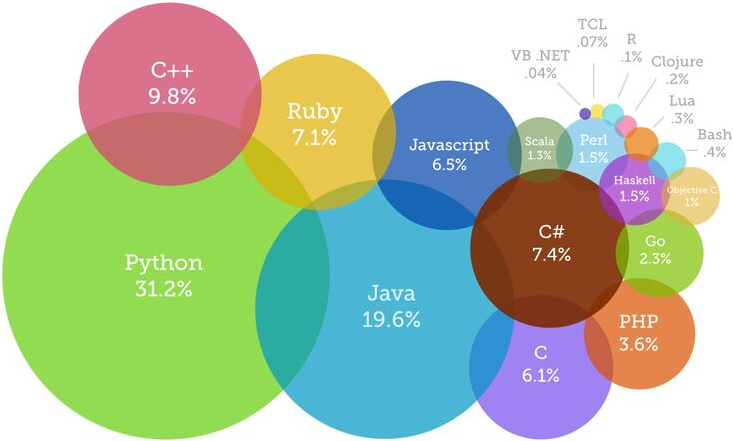
\includegraphics[width=7cm]{ch-langages/img/languages.png}\\ \scriptsize   Langages les plus appris en 2019.\\
    Source : \texttt{learnworthy.net}.
\end{center}
\section{\'Evolution au cours du temps}


Les progrès réalisés sur les analyseurs de code permettent de créer des langages avec une syntaxe de plus en plus épurée courte et pour lesquels il n'est pas obligé de déclarer le type de chaque variable.\\
Les nouveaux langages s'inspirent souvent de leurs prédécesseurs.\\
    
On continue d'inventer de nouveaux langages : ceux-ci sont crées en fonction des besoins de l'époque.\\
De nos jours, les langages qui permettent de programmer facilement plusieurs tâches simultanées (comme par exemple récupérer des données sur \textsc{Internet} et en même temps traiter ces données) ont le vent en poupe.

\begin{center}
    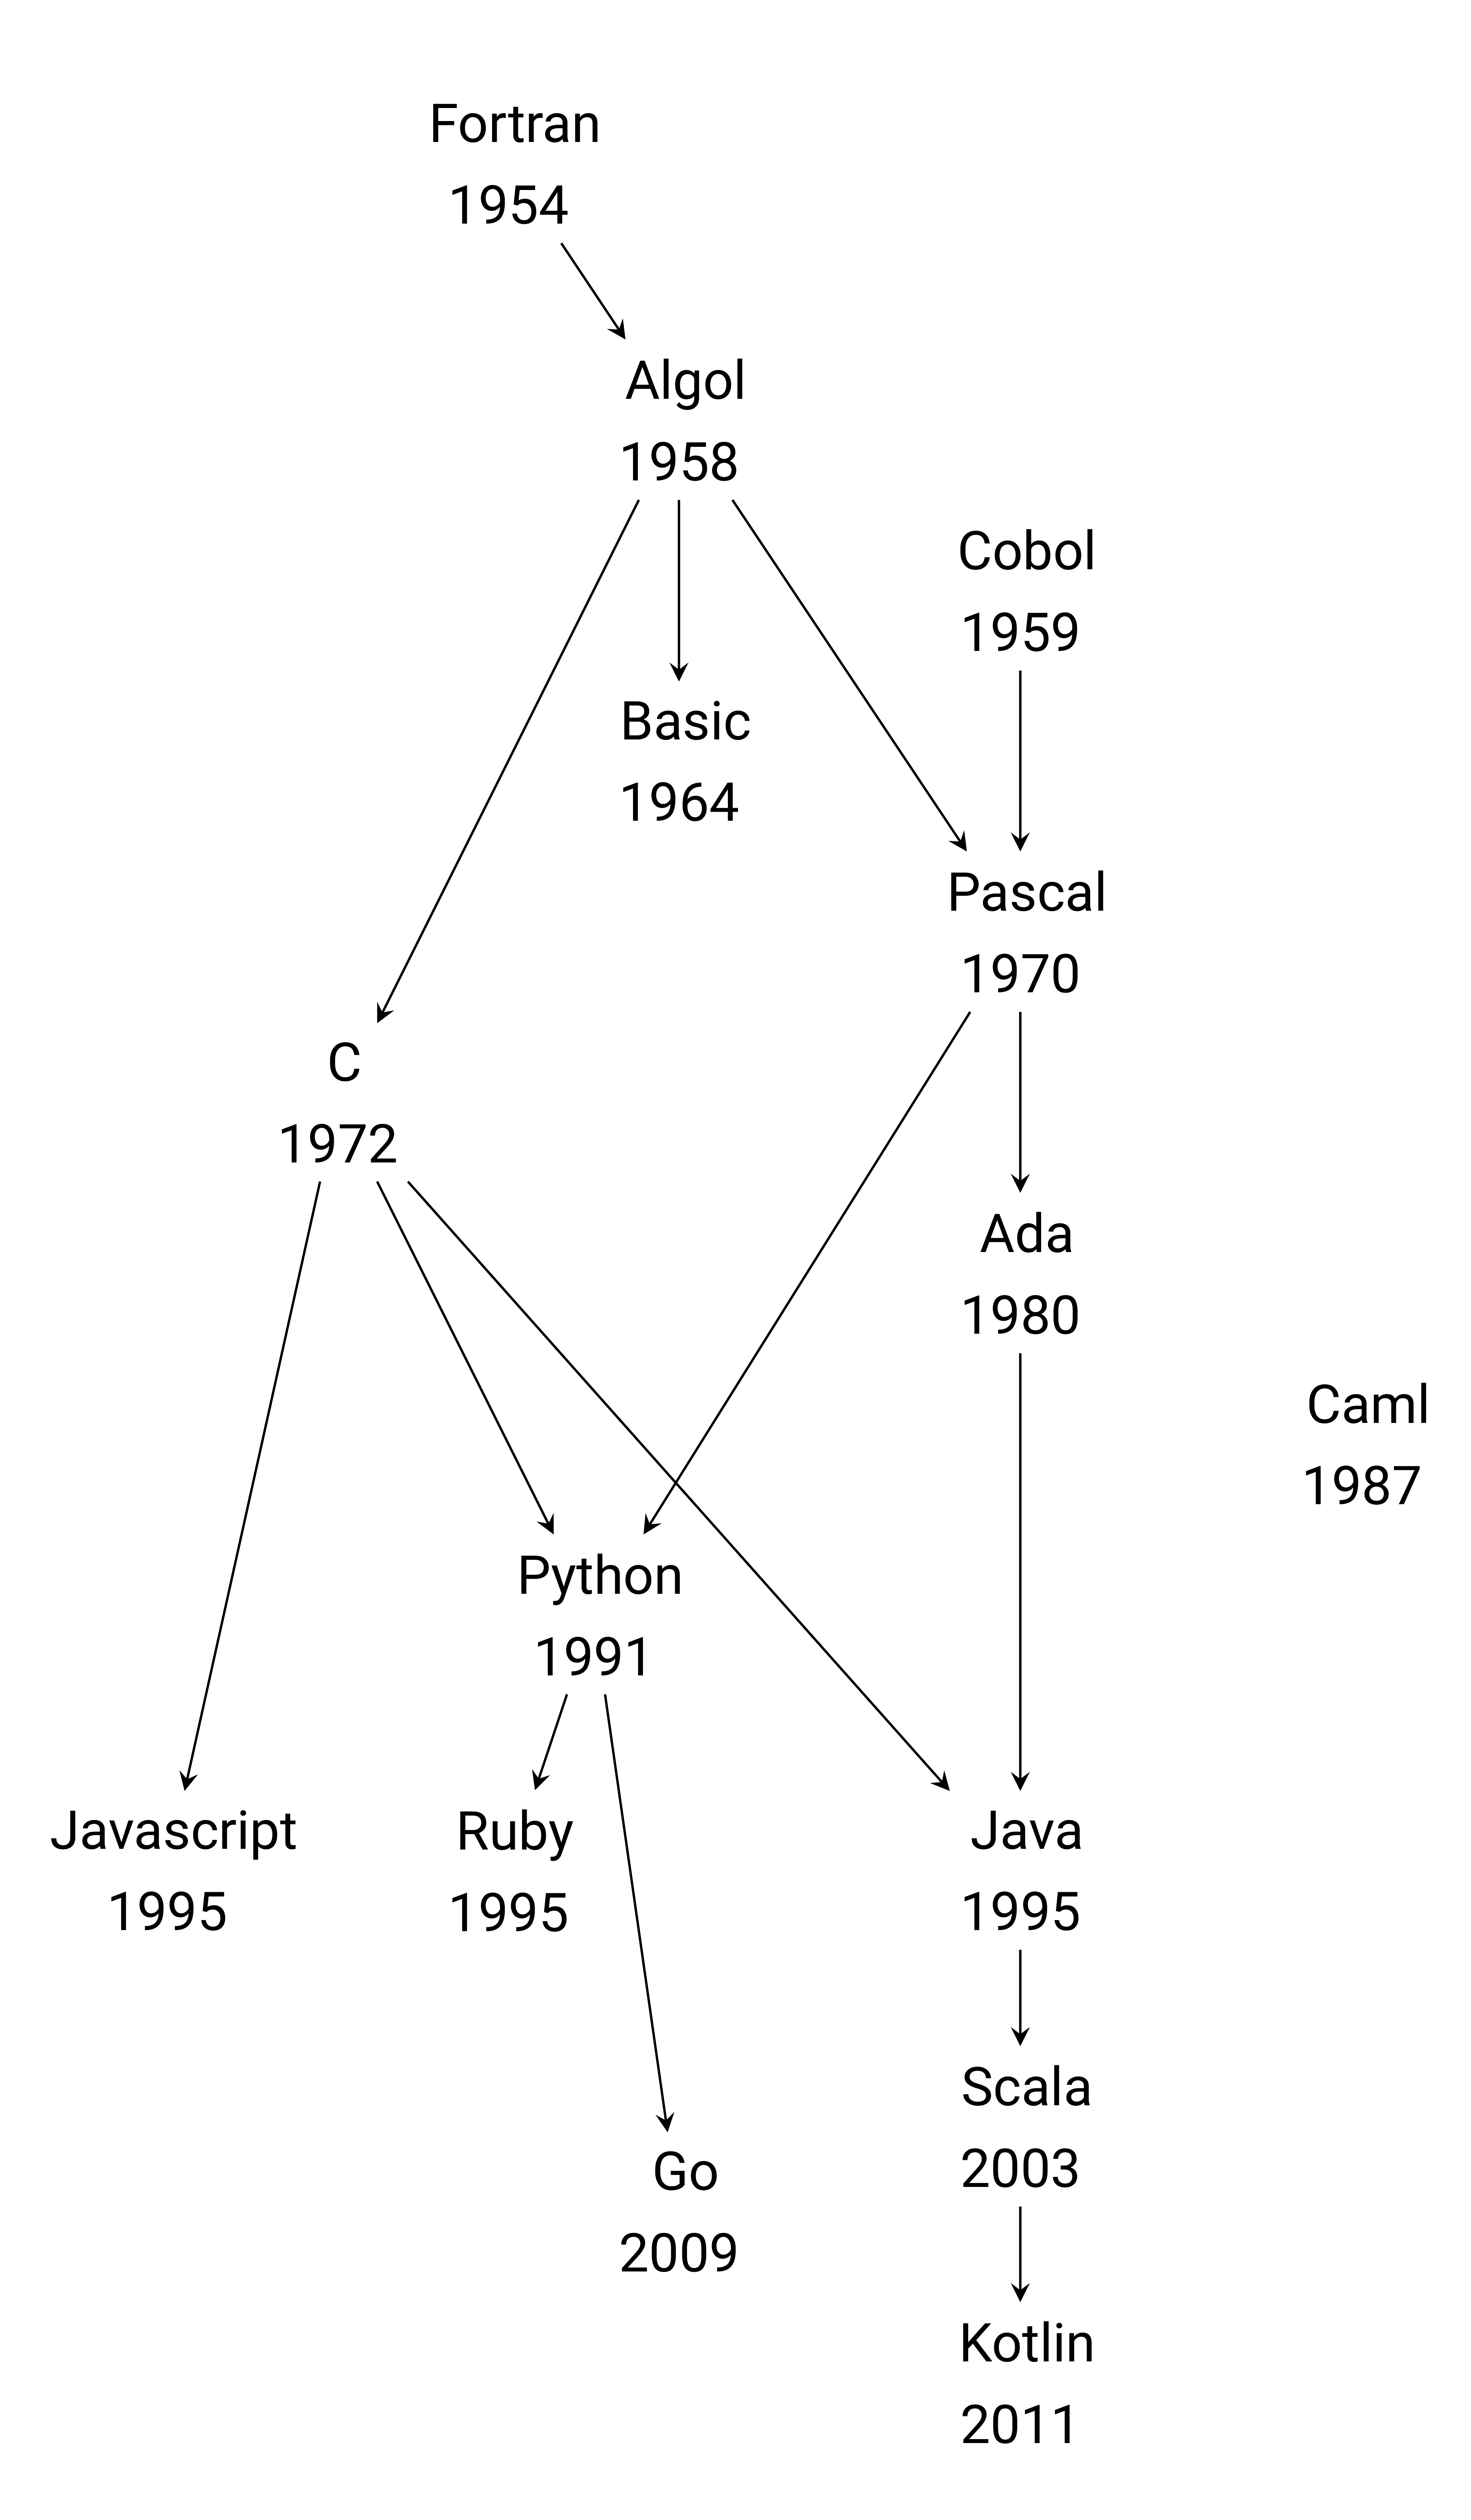
\includegraphics[width=5cm]{ch-langages/img/genealogie.png}\\ \scriptsize   Voici un graphe indiquant comment les langages anciens ont influencé les nouveaux.\\
\end{center}
\ \\[3em]



\begin{center}
    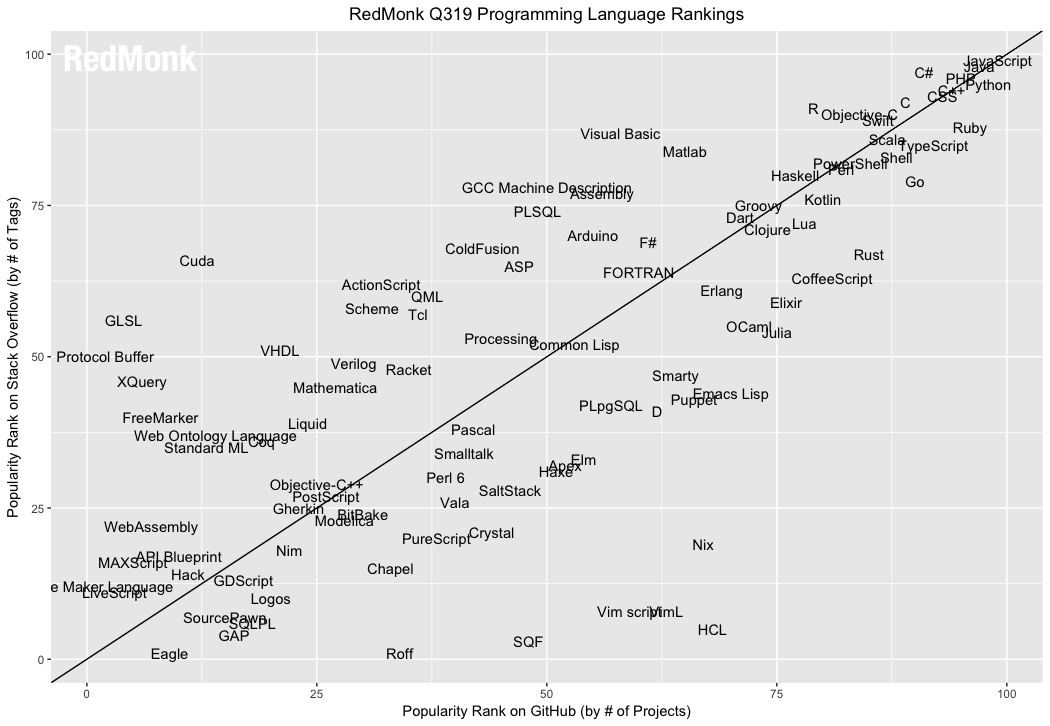
\includegraphics[width=7cm]{ch-langages/img/rank.png}\\ \scriptsize    \textit{Stack Overflow} est un forum d'entraide à la programmation.\\ \textit{GitHub} est un service d'hébergement de projets logiciels.\\
    Le graphique suivant indique la popularité de différents langages sur ces deux sites.\\
    Source : \texttt{redmonk.com}.
\end{center}
